\section{Privacy Provenance Overview}
This section explores how provenance information can be leveraged to enhance the effectiveness of DP systems. We introduce the concept of \emph{DP provenance}, a systematic approach to capture and utilize provenance to support DP systems. We propose a new taxonomy that categorizes existing work based on the type and granularity of the provenance considered. We then delve into how different types of provenance can be used to improve various aspects of DP systems.

\subsection{DP System Model: A Provenance Perspective}
\label{sec:dpsystem}
Every data system that integrates DP has to record and track some additional metadata, compared to that without DP.
We start with a simple, hypothetical system with DP to show the most basic functionalities and the coarsest privacy provenance tracking provided by it.
We then lay out the different entities/components of a DP system that motivate the need for finer-grained privacy provenance or additional provenance features.

\stitle{A (Hypothetically) Basic DP System.}
Consider running a DP system in the central setting, where a \emph{trusted data curator} maintains a protected database $D$.
The data curator sets up a finite \emph{system-wise or global privacy budget} to bound the overall extent of information disclosure \emph{over this database}.
(A group of) untrusted data analyst(s) would like to query the private database $D$.
Each incoming query from a data analyst specifies a \emph{per-query privacy budget} that indicates the amount of budget they would like to spend on this particular query. 
The DP system uses \textit{a fixed mechanism} (e.g., the Laplace mechanism) to answer this query, and subtracts the per-query privacy budget from the global budget.
The system rejects a query if the remaining global budget is not sufficient for this query; it stops processing queries once the global privacy budget is fully depleted.

This basic system can only support limited queries (that could be na\"ively answered through one fixed mechanism). 
Almost every DP system that researchers implement in literature is more complicated than it.
Even though, the basic system has to track the privacy loss in terms of the per-query privacy budget and the global budget consumption\footnote{Indeed, in real-world implementations which lack careful management, DP can rapidly become excessively restrictive so that service providers have to set up a large (or even infinite) global budget, which has been shown to attacks~\cite{tang2017privacy}.
}, which is the simplest example of privacy provenance.
This oversimplified setting overlooks the complexity of a real-world DP system.
Next, we will provide a view of the complexity of system designs for real-world DP systems.

\stitle{The Complexity of DP Systems.}
The design of a DP system greatly depends on the users's role, interest, and expertise levels in this system. First, the data analysts (who are the queries or the programmers) of a DP system have no direct access to the data. They care for the accuracy of the query results and how many queries they can interact with the system. Ideally, if the data analysts have the full domain knowledge of DP and how the system works, then they can understand the DP programs supported by the systems and trace the necessary meta information for optimizing their interested queries. If not, they may not be able to specify the privacy budget correctly and understand the noisy outputs.
A usable DP system in practice is expected to accommodate the needs of both types of data analysts. 
It should explain the noisy output to DP novices and provide modularized APIs for DP experts to program their own tasks.

Second, the data curators are responsible for setting up the data input for the programs and allocating privacy budgets among different analysts.
The basic DP system makes several assumptions to simplify the privacy analysis.
It assumes that the database is static (i.e., not subject to updating), and each row in the database corresponds to a single individual.
In addition, the privacy analysis is rigidly enforced at the entire table level, and the protection is uniform across every row in the database.
In real-world use cases, however, the underlying database is often under dynamic changing and has the hetergenous nature that not every part of the data is equally sensitive.
For example, new data analysts can keep opt-in, and their data will be merged into the private database when the system is running.
The data contributors may have different contributions to the database in terms of the number of rows.
They may also have personalized opinions or different privacy awareness regarding the protection of their data.
In such scenarios, keeping a single global privacy budget and simple privacy analysis at the table level is not sufficient to provide the desired level of privacy guarantees.
In addition, data analysts can have different trust or privilege levels when accessing the system. Tech companies, for example, need to query their users’ data for internal applications like anomaly detection. 
They also consider inviting external researchers with low privilege levels to access the same sensitive data for study through the shared query interface.
It is unfair if a data analyst with a low privilege level asks queries with a significant portion of the global budget so that higher privileged analysts have no more budget to consume.
Therefore, a real DP system involving multiple data analysts may have a range of design choices to make, from privilege allocation to query/task scheduling to assumptions on whether the analysts can collude, etc.

Third, the DP programs responsible for mapping the utility interests of data analysts and the privacy interests of data curators have a wide range of complexities. Some have a fixed query template with a deterministic sensitivity and hence noise scale (e.g., stability tracking in PINQ~\cite{mcsherry2009pinq}); some require dynamic sensitivity analysis (e.g., query rewriting in Chorus~\cite{johnson2020chorus}); and most systems deal with more than one query~\cite{mcsherry2009pinq,johnson2020chorus,ge2019apex,ebadi2015differential}. The queries to be supported can be complicated, e.g., involving multiple transformations of data, and be batched into an OLAP workload.
The desirable system should support multiple mechanisms (including customized ones) to answer different types of queries and additional algorithms to choose among the mechanisms to optimize the privacy-utility trade-off for the queries (especially for the workloads).


In every stage/aspect of the DP system, we have observed evidence or challenges that the basic DP system or coarse-grained DP provenance cannot address.
We envision that a framework with \textit{fine-grained privacy provenance} can help solve these challenges and ensure a more usable and optimized DP system for practical needs, which is described next.


\subsection{The Taxonomy of Fine-Grained Privacy Provenance}

We draw an analogy to provenance in databases and, similarly, characterize the privacy provenance into three categories: ``why-DP-provenance'' (or output-provenance), ``how-DP-provenance'' (or process-provenance), and ``what-DP-provenance'' (or input-provenance), based on the information/metadata they track and the aspects they influence a DP system.

\begin{table}
    \centering
    \caption{Comparison between different types of provenance in databases~\cite{cheney2009provenance} and privacy provenance.}
    %\begin{adjustbox}{width=1\textwidth}
    %\scriptsize	
    \begin{tabular}{p{3.9cm}|p{5cm}|p{6cm}}
    \toprule\hline
         & \textbf{Database Provenances~\cite{cheney2009provenance}} & \textbf{Privacy Provenances} \\ \hline
      Why-(DP-)Provenance   & {Identifying sub-instances of the input that ``witness'' a part of the output}  & Explaining why a noisy output satisfies accuracy requirements and/or why certain queries are rejected  \\ \hline
      How-(DP-)Provenance   & Providing additional information on how the output tuple is derived, e.g., transformations applied during processing & Tracing query metadata for tighter privacy analysis during executing DP program/mechanisms (that are complex or involving multiple data analysts) \\ \hline
      Where-(DP-)Provenance   & Pinpointing where an attribute value in the output tuple is exactly copied from & Managing budget consumption for heterogeneous private input data sources (e.g., user-level DP, personalized DP) \\ \hline \bottomrule
    \end{tabular}
    %\end{adjustbox}
    \label{tab:comp_prov_dp}
\end{table}

% \begin{figure}
%     \centering
%     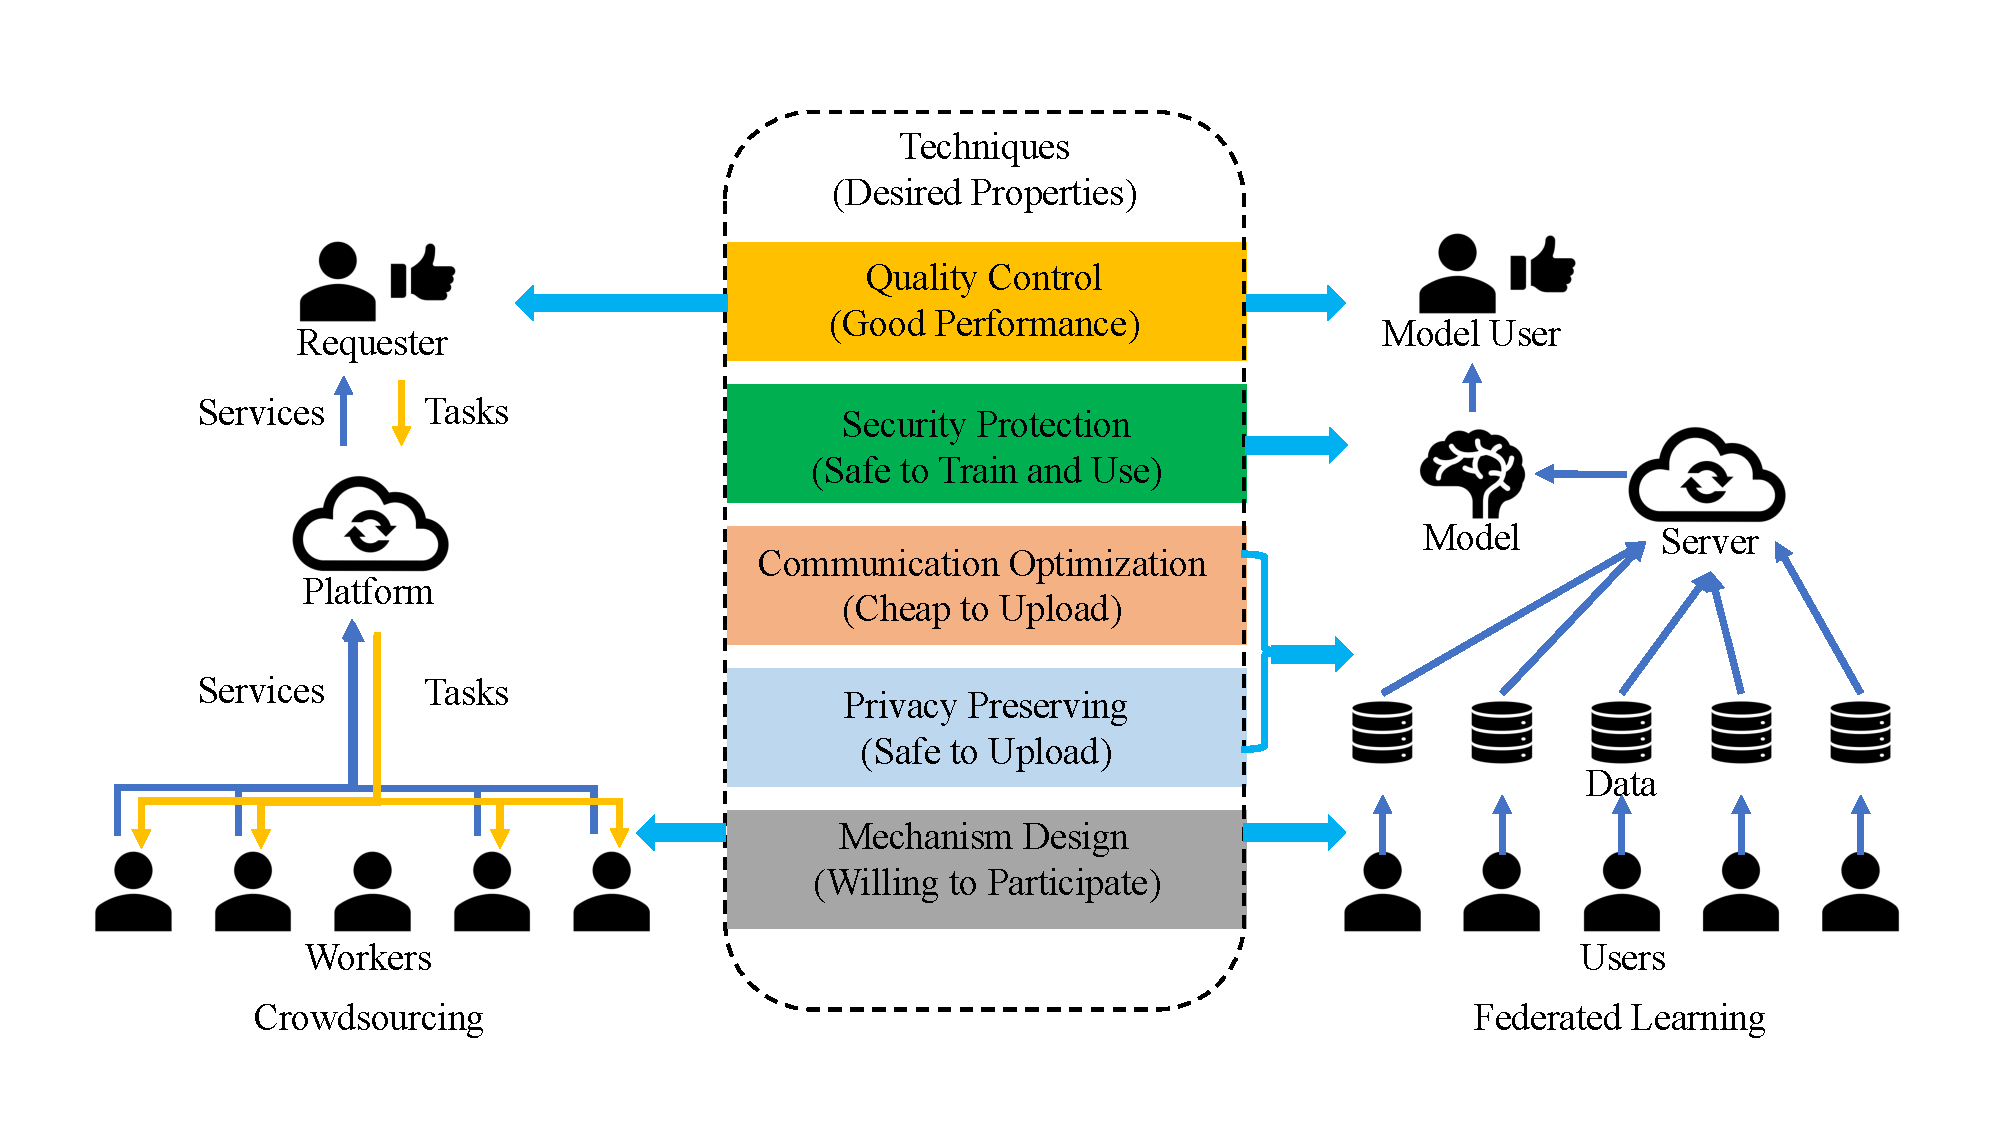
\includegraphics[width=\textwidth]{figs/comparison.png}
%     \caption{Caption}
%     \label{fig:enter-label}
% \end{figure}


\stitle{Why-DP-Provenance}, also known as output-provenance, refers to the additional information that helps data analysts understand the reasoning behind a DP system's output. It focuses on the interaction between the system's results and the analyst's needs.
Why-DP-provenance aims to answer questions like, \emph{why is a specific privacy budget chosen for the analyst's query, how does the level of noise in the answer achieve the desired accuracy, why is a noisy answer still considered useful, and what factors lead to a query rejection?}
Benefits of enforcing fine-grained why-DP-provenance include:
\begin{itemize}
    \item \emph{Explainability and Interpretability}: Why-DP-provenance details query answers' usefulness and confidence intervals, which allows analysts to understand the trade-offs between privacy guarantees and accuracy.
    \item \emph{Tighter Privacy Composition:} Why-DP-provenance facilitates a more accurate understanding of how different queries impact the overall privacy budget. \item \emph{Optimal Privacy-Accuracy Trade-Offs:} Why-DP-provenance empowers analysts to make informed decisions about the balance between privacy and the usefulness of results. 
\end{itemize}
Techniques for why-DP-provenance device approaches for accuracy-first query specification, error specification, fine-grained budget specification, and others.
Unlike the why-provenance in databases that focuses on ``why'' something happened or exists, the why-DP-provenance answers ``why'' a specific level of parameters in a DP algorithm is chosen and its impact on results within a DP system.





\stitle{How-DP-Provenance}, also known as process-provenance, focuses on capturing details about the specific privacy mechanisms employed within a DP system. This information becomes crucial for answering complex queries privately, building complex DP mechanisms, or selecting the optimal/best DP mechanisms for a query workload.
How-DP-provenance solves the following questions: \emph{How is the noise for a private query calculated based on a series of transformations of data? What structural properties of a query can be used for a tighter privacy bound? Can we reuse the noise calibrated to historical queries for answering new queries to save the privacy budget?}
Fine-grained how-DP-provenance tracking enables: 
\begin{itemize}
    \item \emph{Efficient Privacy Analysis:} How-DP-provenance tracks the series of modularized transformations or the query structural properties for complex queries to make sensitivity analysis more efficient.
    \item \emph{Better Utility for Query Workloads:} How-DP-provenance reuses noise from historical query answers or injects correlated noise to a batch of queries to increase the overall utility for the workload.
    \item \emph{Effective Budget Allocation:} How-DP-provenance facilitates the budget allocation across multiple data analysts so that the privacy loss is tightened when analysts collude.
\end{itemize}
Techniques that support fine-grained how-DP-provenance include transformation tracking and noise tracking.
Different from the how-provenance in databases that generates a derivability relationship between output and input tuples, the how-DP-provenance answers ``how'' a better DP mechanism could be designed or modularized for answering queries.



\stitle{Where-DP-Provenance}, also known as input-provenance, accounts for which (part of) private input data is used for a DP mechanism.
The complex data type can involve multiple database tables, and queries over different tables can result in different DP guarantees --- tracking which tables are used for what queries becomes essential for multi-relational DP systems.
Furthermore, even with a single table, different queries or mechanisms may be interested in different parts of the table --- accounting privacy loss at the table-level can waste more privacy budgets.
Third, data may be merged at different timestamps or belong to different users.
Thereby, where-DP-provenance tracks privacy loss for data by answering questions of \emph{what part of the private data is used to answer a particular query, what (group of) users are associated with the data.}
With where-DP-provenance, the system gains:
\begin{itemize}
    \item \emph{Flexibility with Multi-Resolution Privacy}: Where-DP-provenance allows data curators to specify policies with different resolutions of privacy guarantees.
    \item \emph{Continuously Running System}: Where-DP-provenance enables the replacement of retired data with new data so that the system can continuously execute.
\end{itemize}
While the where-provenance in databases pinpoints the exact places that an output tuple is copied from, the where-DP-provenance answers ``where'' incurs a privacy loss in the private input w.r.t queries.





Next, we will describe the DP techniques that fit into the framework of each why, how, and where-DP-provenance and the different granularities of these techniques.


\subsubsection{Techniques for Why-DP-Provenance}


\stitle{Query Specification.}
Two types of DP query specification exist: \emph{privacy-first} and \emph{accuracy-first}.
Most (traditional) DP building blocks or systems are \emph{privacy-first}, meaning that they require the data analysts to specify a privacy budget for their queries or tasks to run.
This privacy budget will be deducted from the global privacy budget if the tasks are executed and the noisy answers are returned to the analysts.
While this approach is easy to analyze and has many optimal and off-the-shelf mechanisms developed over the years, it may limit the usability of a DP system: the data analysts care about the quality of the query answers, but may not have sufficient expertise to understand the DP mechanisms and the relationship between privacy and the error rate according to the chosen mechanism.
Since a DP system cannot release the true query answer, a single noisy output cannot explain how well the black-box mechanism works to privacy novice analysts.
In addition, the released answers (or consumed budget) can not be reversed—discarding unsatisfactory query answers simply wastes the global privacy budget.


Another approach for query specification is \textit{accuracy-first}~\cite{ge2019apex,Ghayyur2022mide,dprovdb,WhitehouseRWR22brownian,xiao2021optimizing,ligett2017accuracy,mazmudar2022cache,pioneer}, that allows the data analysts to superimpose an accuracy requirement in the query specification, and the system can translate the accuracy requirements into privacy budget and automatically choose the optimal mechanism to answer this query.
This approach aims to close the discrepancy between privacy-oriented DP mechanisms and the needs of data analysts for understanding noisy outputs, but many open problems remain in understanding data-dependent accuracy translation.
Recent work like DPella~\cite{lobo2020programming} and DProvDB~\cite{dprovdb} support both the privacy- and accuracy-oriented modes.





\stitle{Error Specification.} 
A line of work, including DPComp~\cite{hay2016exploring}, Overlook~\cite{thaker2020overlook}, PSI~\cite{gaboardi2016psi}, Bittner et al.~\cite{bittner2020understanding}, DPP~\cite{john2021decision}, ViP~\cite{NanayakkaraB0HR22visualizing}, and DPXPlain~\cite{TaoGMR22DPXPlain}, aims to provide interfaces for explaining the noisy output to the data analyst or visualizing an optimal privacy-utility trade-off due to the mechanism to help the analysts make informed choices.
These tools explore a DP confidence interval of the noisy answer~\cite{covington2021unbiased,du2020differentially,cohen2023optimal,drechsler2022nonparametric,NanayakkaraB0HR22visualizing,SunDY23CI} or other statistical metrics on measuring accuracy of the answer as functions of the selected privacy budget~\cite{thaker2020overlook,john2021decision}.
ViP~\cite{NanayakkaraB0HR22visualizing} associates the query output with a differentially private randomization interval, indicating the noise bounds of the query result with high confidence.
This randomization bound could be either post-processed from a noisy answer if the mechanism is data-independent or computed with a small portion of additional privacy budget from data-dependent mechanisms~\cite{covington2021unbiased,du2020differentially,cohen2023optimal,drechsler2022nonparametric}.
DPXPlain~\cite{TaoGMR22DPXPlain}, on the other hand, start to explore methods of providing additional explanation of aggregation query results, on which whether an unexpected answer is due to the data itself or the randomness introduced by DP.
 
\stitle{Budget Specification.} 
The composition of privacy loss through a series of queries can be classified into two levels, based on whether different analysts are distinguished.
The coarser level of query composition is to regard all data analysts as a unified entity, and the system sequential composition to account for privacy loss during the execution of the queries.
This method is easy to implement, well-suited to different types of (complex) queries, and can explain whether a query is rejected—the privacy budget or the translated privacy budget exceeds the remaining global privacy budget.
Sequential composition can also be replaced by a privacy odometer~\cite{RogersVRU16odometer,lecuyer2021odometer} or adaptive composition~\cite{whitehouse2023fully,winograd2017framework,kairouz15} that gives tighter privacy bound over the queries that are adaptively asked, but they are restricted to simple queries.
More fine-grained query composition is to track the privacy loss as per data analysts and per queries they ask~\cite{dprovdb}.
This approach can not only answer more specific questions on \textit{why this particular analyst's query is rejected} but also achieve fairness among multiple data analysts when they are assigned different trust/privilege levels.
However, fine-grained tracking requires recording more metadata proportional to the number of data analysts in the system.


\stitle{Other Techniques for Why-DP-Provenance: Automated DP Proof Generation.}
Besides explaining noisy output to the data analysts, another line of work investigates the logical representation and execution of a differentially private mechanism/system.
They check and verify the privacy properties of a DP program implementation by either generating automated proofs for DP~\cite{wang2021dpgen,abuah2021dduo,wang2020checkdp,wang2019proving,zhang2017lightdp,near2019duet,solo22} or detecting counterexamples that violate DP guarantees~\cite{ding2018detecting,bichsel2018dp,bichsel2021dp,barthe2020deciding} through annotated type systems and static/dynamic analysis of the program execution.



\subsubsection{Techniques for How-DP-Provenance}

\stitle{Transformation Tracking.}
Complex database queries often consist of a series of transformations over the private data, e.g., selection, projection, group-by, join, union, and aggregation. 
In order to calibrate noise to the query answers, the system needs to analyze the sensitivity of the query.
We categorize the approaches to estimate the sensitivity of a query into three levels, from coarse-grained to fine-grained: tracking sensitivity directly, tracking transformation stability, and tracking query structures.

\noindent
\emph{Tracking Sensitivity (Directly).}
The coarsest level of how-DP-provenance is to directly compute an upper bound of the query sensitivity.
For simple queries, the sensitivities are well understood and can be computed easily.
However, for complex queries, without making clever use of the properties of the query, the sensitivity could be overestimated or cumbersome to compute.

\noindent
\emph{Tracking Transformation Stability.}
Existing systems like PINQ~\cite{mcsherry2009pinq} and wPINQ~\cite{ProserpioGM14wpinq} keep track of the \textit{transformation stability} to calculate the amount of noise needed for the queries.
For a transformation $T: \mc{D} \rightarrow \mc{D}$, it is $c$-stable if $\forall$ two input databases $D, D' \in \mc{D}$, we have $| T(D) \triangle T(D') | \leq c \times |D \triangle D'|$, where $\triangle$ denotes the symmetric difference between two databases, i.e., $D \triangle D' = (D \backslash D') \cup (D' \backslash D)$.
For example, common SQL transformations selection, projection, and counting queries have stability of 1, and group-by has a stability of 2.
It has been shown that for a $\epsilon$-differentially private mechanism $\mc{M}$ and a $c$-stable transformation series $T$, the composition $\mc{M} \circ T$ will be $(c \cdot \epsilon)$-differentially private.


\noindent
\emph{Tracking Query Structures.}
Keeping the transformation stability metadata makes it easy to analyze the privacy loss for a series of linear transformations before histogram queries, but may not be sufficient for highly sensitive queries like aggregation and join.
The query sensitivity for aggregations could be as large as the size of the domain product (e.g., sum over selected attributes).
The approach to handling aggregation queries is to truncate the attribute domain~\cite{johnson2020chorus,FangD022shifted,dong2023universal} and/or perform aggregations on disjoint subsamples~\cite{nissim2007smooth,mohan2012gupt,Smith11sample_aggregate,johnson2020chorus}, which requires the system to keep track of the truncation information per query and per attribute and the information about how the truncation transfers over queries.
Chorus~\cite{johnson2020chorus} enables a query rewriting and annotation technique, which could be seen as using \textit{how-DP-provenance}, to automatically trace and analyze the query stability and truncated domain when processing aggregation queries.
Similarly, the sensitivity of join queries can be even unbounded — changing one tuple in an input table can cause unbounded changes in the join output since this tuple can match an arbitrary number of tuples in another input table.
DP mechanisms for answering join queries clip the maximum number of tuples that a tuple can match in a join~\cite{kotsogiannis2019privatesql}, or add data-dependent noises~\cite{nissim2007smooth,johnson2018towards,dong2021residual,dong2021nearly}, or a mixture of both~\cite{dong2022r2t}.
Indeed, the recent residual sensitivity mechanism~\cite{dong2021residual} analyzes the multi-way join topology metadata and traces a smooth upper bound of local sensitivity across this join topology to \textit{efficiently} calculate a \textit{tighter} noise.


\stitle{Noise Tracking.}
While the basic DP system does not track the noise added to each query answer (i.e., queries are regarded as independent), a number of recent work~\cite{dprovdb,mazmudar2022cache,xiao2022answering,li2014data,hardt2010multiplicative,KostopoulouTCGL23turbo} inject correlated noise to the answers.
They optimize the accuracy of the query results by batching the query workload and adding correlated noise with the \emph{workload of one single data analyst}~\cite{xiao2021optimizing,li2014data,dong23composition}, or, in a more fine-grained way, maintaining a stateful cache of the historical query answers~\cite{mazmudar2022cache,KostopoulouTCGL23turbo,kotsogiannis2019privatesql} so that answers to the new queries can reuse the cached noises.
The DP caches are extended from answering one data analyst's queries to mitigating privacy loss across multiple data analysts~\cite{dprovdb,DworkNV12power_of_state,nicolas2023cohere,HsuRU13equilibrium} or tight adaptive composition~\cite{vadhan2021concurrent,vadhan2023concurrent} across analysts when multiple analysts ask the same or similar queries.
Other multi-analyst systems~\cite{xiao2021optimizing,xiao2022answering,knopf2021framework,pujol2021budget,pujol2022multi} tracks per-analyst privacy \cite{xiao2021optimizing} or accuracy \cite{knopf2021framework} constraints to optimize the privacy-accuracy trade-off or fairly answer queries among analysts \cite{pujol2021budget,pujol2022multi}.
Among all the different settings in multi-analyst DP, additional fine-grained requirements or privacy guarantees regarding different analysts' queries are recorded for the DP mechanism designs, which is in line with how-DP-provenance.



\subsubsection{Techniques for Where-DP-Provenance}

\stitle{Privacy Resolutions.} 
Depending on the data model and the intended privacy goals to deliver, a DP system can achieve the notion of \textit{event-level DP}, \textit{user-level DP}, \emph{multi-resolution DP} (defined as per policies)~\cite{he2014blowfish,kotsogiannis2019privatesql} and other extended notions of DP, e.g., personalized user-level DP~\cite{jorgensen2015personalized}.
Event-level DP assumes that in the private input data, each individual contributes only one record, while it is a special case of user-level DP, which allows each individual to make multiple contributions and reasons about privacy at the user level.
In particular, the neighboring database definition is different in the two settings, which changes the way sensitivity is analyzed.
Other DP notions, such as Pufferfish privacy~\cite{kifer2014pufferfish}, Blowfish privacy~\cite{he2014blowfish}, multi-resolution privacy~\cite{kotsogiannis2019privatesql}, per-attribute DP\cite{Ghazi0M023per_attr_DP}, Metric DP~\cite{chatzikokolakis2013broadening}, geo-indistinguishability~\cite{yu2022thwarting}, etc., relax and extend DP to more general settings for example with correlations.


\stitle{Privacy Accounting.} 
Accounting for privacy loss over the input data is challenging.
The basic DP system performs the privacy composition at the table level.
However, it is unlikely that every query touches the entire table.
Accounting privacy at the table level would waste privacy budgets for the part of data that is not used for computations.
More fine-grained privacy accounting considers splitting databases into disjoint blocks and sub-tables, and only the block that is used for answering a query will be deducted for privacy consumption.
This approach is called parallel composition or block composition~\cite{mcsherry2009pinq,LecuyerSVG019sage}.
This has also been extended in recent work~\cite{nicolas2023cohere} that a finer-grained user-level partitioning is available at the column level so that the wasted privacy budget can be minimized.
Other than privacy accounting for different parts of the data, the input data can arrive at different timestamps.
Based on the DP models used, existing work proposes mechanisms for sliding windows~\cite{kellaris2014differentially}, the entire streams~\cite{DworkNPRY10panprivate,dong2024continual,DongLY23continual} or with historical data~\cite{growingdb18}.




\begin{table}
\caption{Taxonomy of Privacy Provenance and Evaluations of Implemented DP Systems. \cmark=with, \xmark=without, \Circle=Coarse-Grained, \LEFTcircle=Moderate-Grained, \CIRCLE=Fine-Grained. Shaded rows indicate systems surveyed in case studies. 
}
\scriptsize	
%\begin{adjustbox}{width=1\textwidth}
    \begin{tabular}{@{}llclllll@{}}
        \toprule
        \multirow{2}{*}{Systems} & \multicolumn{3}{c}{Why-DP-Provenance}                  & \multicolumn{2}{c}{How-DP-Provenance}    & \multicolumn{2}{c}{Where-DP-Provenance} \\ \cmidrule(lr){2-4} \cmidrule(lr){5-6} \cmidrule(l){7-8} & Query Spec     & Err Spec & Budget Spec & Transformation  & Noise (Trackings) & Priv Resolutions    & Priv Accountant   \\ \hline
Basic                    & Privacy-First  & \xmark   & \Circle ~Per Query     & \Circle ~Sens Only          & \xmark ~No            & \Circle ~Event-DP    & \Circle ~Table Level          \\
PINQ~(\citeyear{mcsherry2009pinq})                     & Privacy-First  & \xmark   & \Circle ~Per Query     & \LEFTcircle ~Sens+Stability & \xmark ~No            & \Circle ~Event-DP    & \LEFTcircle ~Sub-Table Level  \\
ProPer~(\citeyear{ebadi2015differential})                   & Privacy-First  & \xmark  & \Circle ~Per Query     & \LEFTcircle ~Sens+Stability & \xmark ~No            & \CIRCLE ~User-DP\textsuperscript{\textdagger}     & \LEFTcircle ~Sub-Table Level \\
PSI$\Psi$~(\citeyear{gaboardi2016psi}) &Privacy-First & \LEFTcircle & \LEFTcircle ~Per Query\textsuperscript{*} &\Circle ~Sens Only & \xmark ~No  & \Circle ~Event-DP & \Circle ~Table Level   \\
$\epsilon${\sc ktelo}~(\citeyear{zhang2018ektelo})   &Privacy-First & \xmark&\Circle ~Per Query& \LEFTcircle ~Sens+Stability & \LEFTcircle ~Workload & \Circle ~Event-DP &\LEFTcircle ~Sub-Table Level \\  
\rowcolor{Gray}                                 
APEx~(\citeyear{ge2019apex})                     & Accuracy-First & \Circle   & \Circle ~Per Query     & \Circle ~Sens Only          & \LEFTcircle ~Workload & \Circle ~Event-DP    & \Circle ~Table Level          \\
PrivateSQL~(\citeyear{kotsogiannis2019privatesql}) & Privacy-First & \xmark & \Circle ~Per Query & \Circle ~Sens Only & \CIRCLE ~Caching & \CIRCLE ~Policy-DP& \Circle ~Table Level\\
\rowcolor{Gray}                                   Sage~(\citeyear{LecuyerSVG019sage})                     & Privacy-First  & \xmark   & \Circle ~Per Query     & \Circle ~Sens Only          & \xmark ~No            & \Circle ~Event-DP    & \LEFTcircle ~Sub-Table Level  \\
Chorus~(\citeyear{johnson2020chorus})                   & Privacy-First  & \xmark   & \Circle ~Per Query     & \CIRCLE ~Query Struct    & \xmark ~No            & \Circle ~Event-DP    & \Circle ~Table Level        \\
CacheDP~(\citeyear{mazmudar2022cache})&Accuracy-First & \Circle&\Circle ~Per Query & \Circle ~Sens Only & \CIRCLE ~Caching & \Circle ~Event-DP & \Circle ~Table Level \\
ViP~(\citeyear{NanayakkaraB0HR22visualizing}) & Privacy-First & \CIRCLE & \LEFTcircle ~Per Query\textsuperscript{*}  & \Circle ~Sens Only  & \xmark ~No & \Circle ~Event-DP & \Circle ~Table Level\\
\rowcolor{Gray}                                 
DProvDB~(\citeyear{dprovdb})                  & Both & \Circle   & \CIRCLE ~Query+Analyst & \LEFTcircle ~Sens+Stability & \CIRCLE ~Caching      & \Circle ~Event-DP    & \Circle ~Table Level          \\
\rowcolor{Gray}                                   Cohere~(\citeyear{nicolas2023cohere})                   & Privacy-First  & \xmark   & \CIRCLE ~Query+Analyst & \Circle ~Sens Only          & \LEFTcircle ~Workload & \LEFTcircle ~User-DP & \CIRCLE ~Column Level         \\


\bottomrule
                                 
        \end{tabular}
%\end{adjustbox}
\flushleft{
\rule{0in}{0em}{ \footnotesize \textsuperscript{\textdagger} ProPer achieves user-level DP with personalized privacy guarantees.}\\
\rule{0in}{0em}{ \footnotesize \textsuperscript{*} ViP and PSI$\Psi$ both support an interface to help analysts split privacy budget across multiple queries. ViP supports more types of error specifications (confidence intervals, quantiles, etc.).}
}
\label{tab:taxonomy}
\end{table}

% \begin{figure}
%     \centering
%     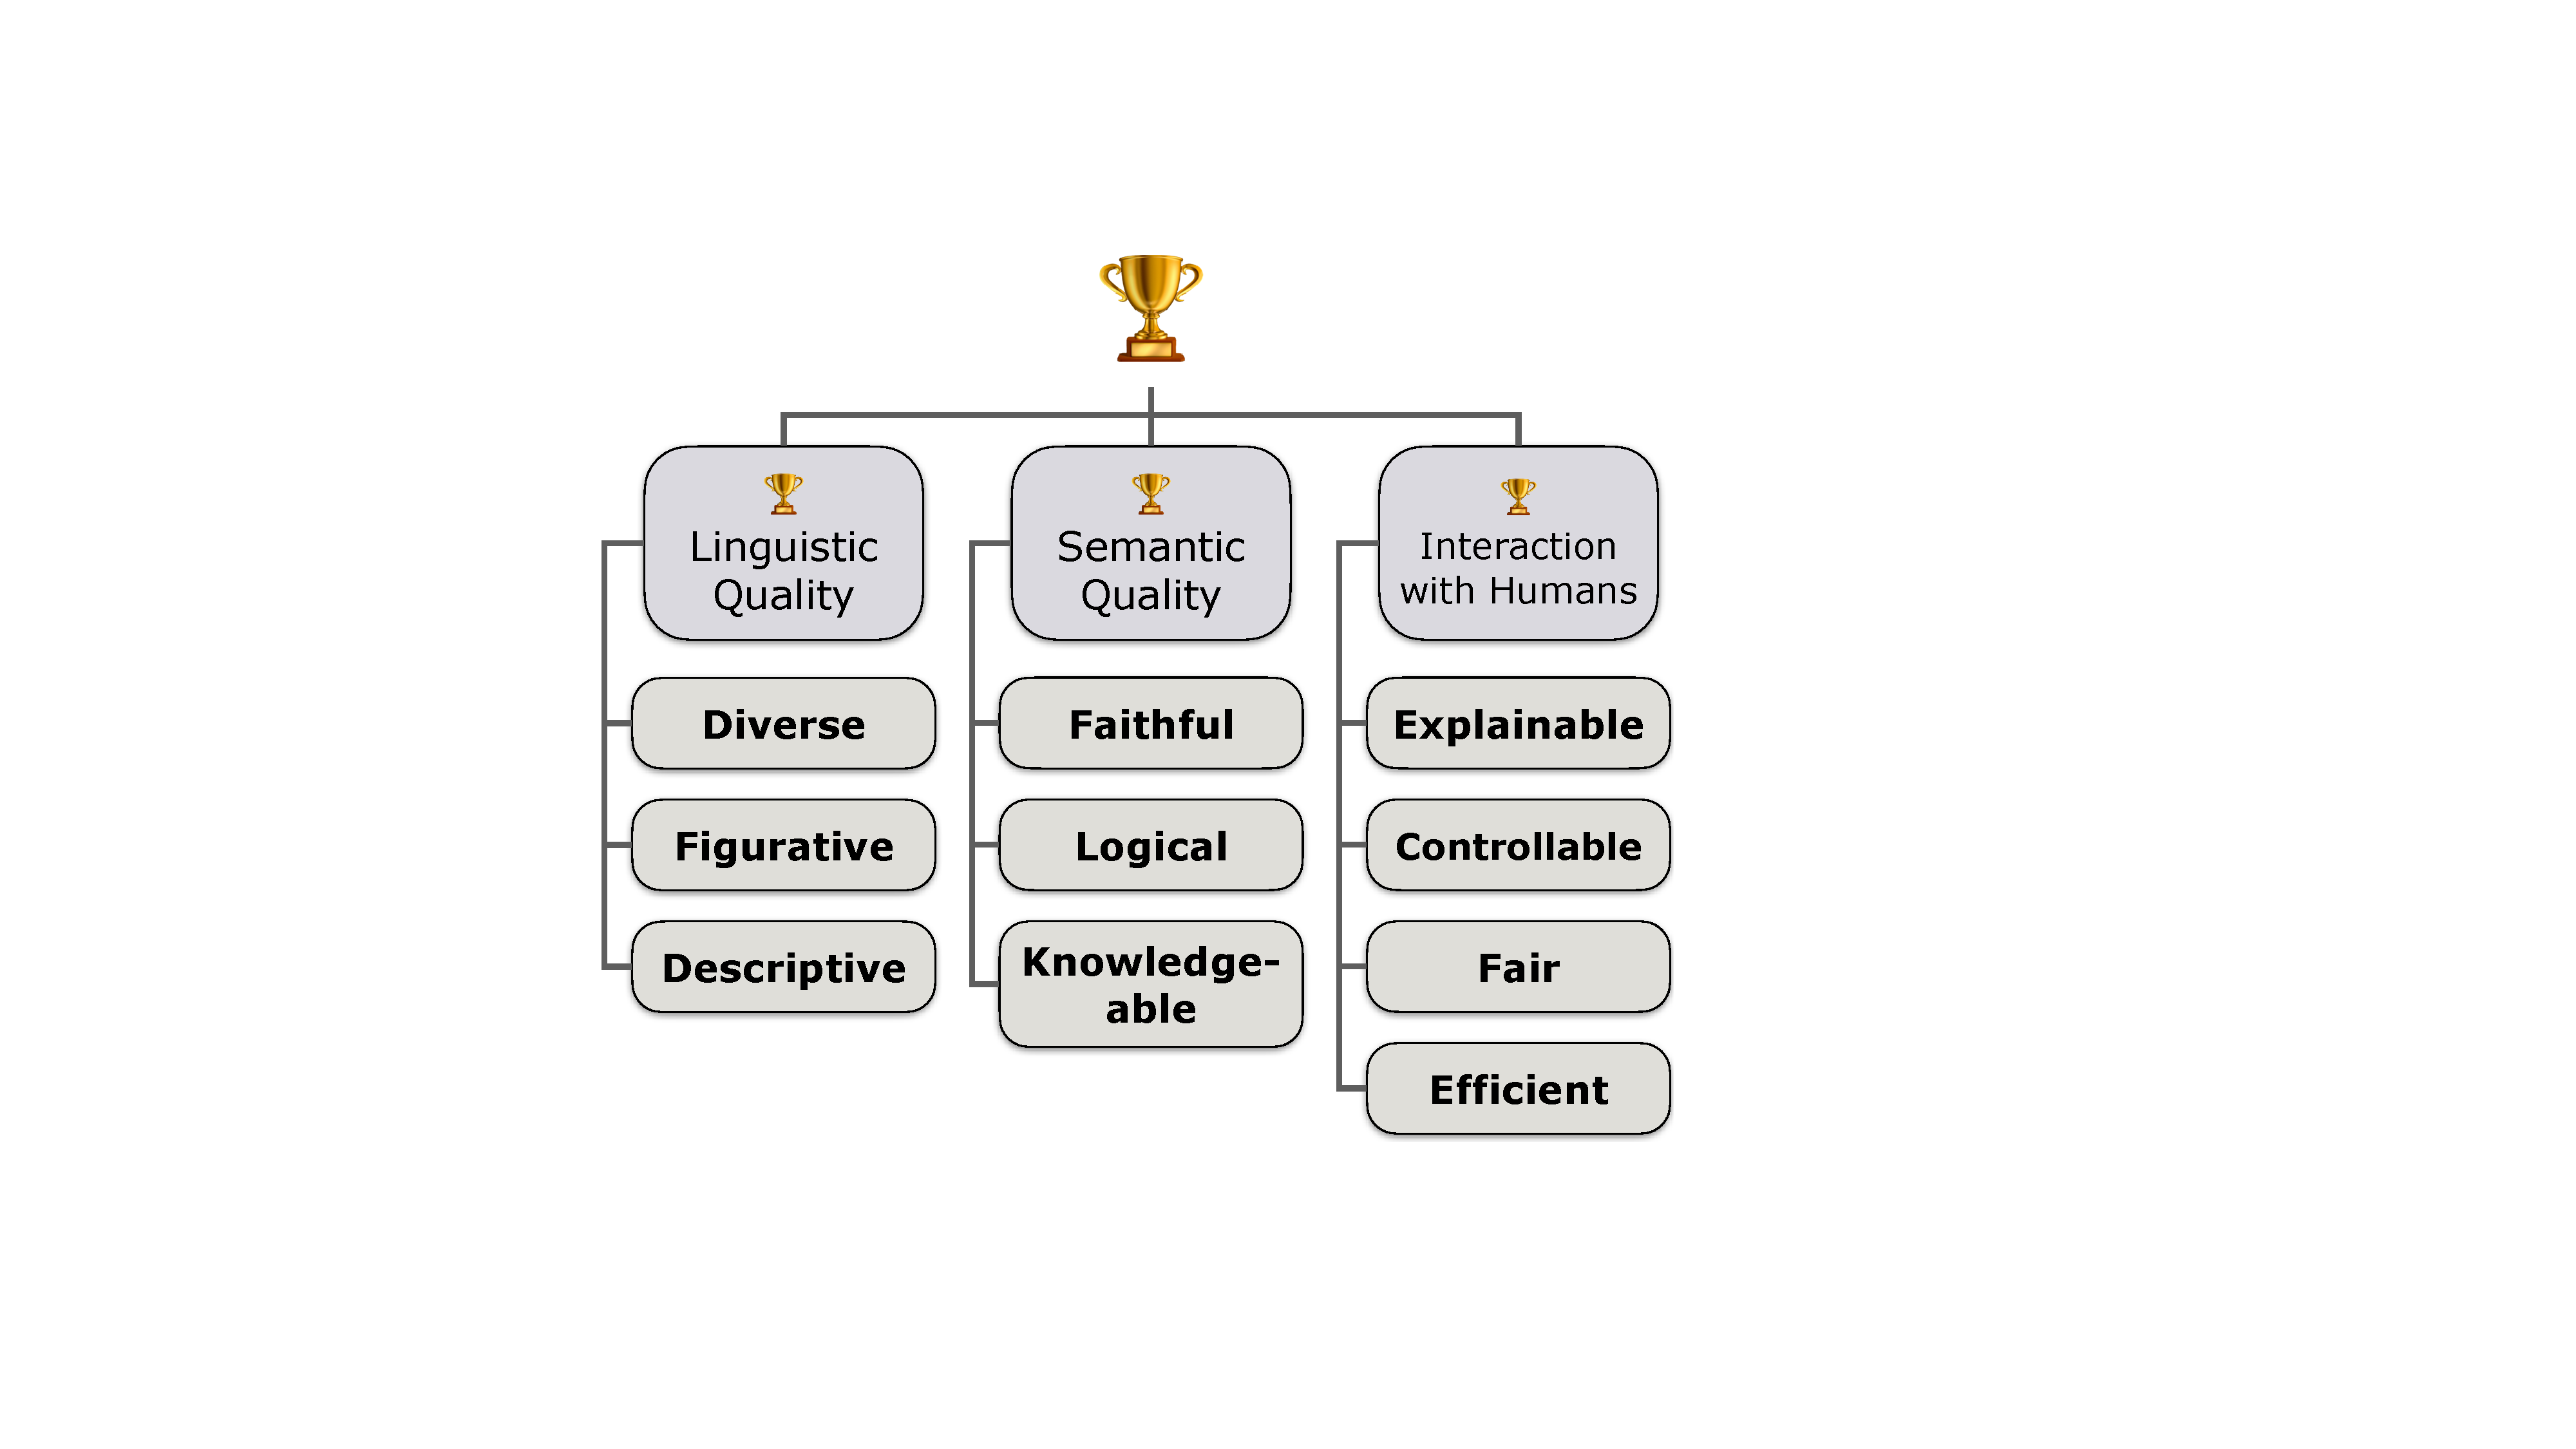
\includegraphics[width=\textwidth]{figs/taxonomy.png}
%     \caption{}
%     \label{fig:enter-label}
% \end{figure}



\bigskip

\noindent
Table~\ref{tab:taxonomy} summarizes the techniques and the granularities of the provenances used in some existing DP systems for DP with trusted data curators (i.e., in the central setting). We discuss other cases that enforce local DP or other models of DP in Section 5.